\documentclass[12pt]{article}

\title{On simulating the four Solar System tests of general relativity using two-parameter post-Newtonian gravitation with Euler integration}
\author{S. Halayka\footnote{sjhalayka@gmail.com}}
\date{\today\;\currenttime}

\usepackage{datetime}
\usepackage{listings}
\usepackage{cite}
\usepackage{xcolor}
\usepackage{graphicx}
\usepackage{setspace}
\usepackage{amsmath}
\usepackage{url}
\usepackage[margin=1.0in]{geometry}

%\doublespace

%\usepackage[]{lineno}
%\linenumbers


\begin{document}



 
\maketitle

\begin{abstract}
A simple numerical solution for general relativity in the Newtonian weak field regime is provided -- no tensor calculus is required.
The topics under consideration are the deflection of photons and neutrinos by the Sun, the relativistic rotation of Mercury's orbit plane, the Shapiro time delay, and the gravitational redshift -- namely, the four Solar System tests of general relativity.
To simplify the calculations, Euler integration is used.
Hopefully, this numerical solution can be found to be an important tool, primarily due to this simplicity.
\end{abstract}


\section{Introduction}

In this paper we will describe a numerical solution for the deflection of photons and neutrinos by the Sun, for the relativistic orbit of Mercury around the Sun, for the Shapiro time delay of photons, and for the gravitational redshift of photons.

No tensor calculus is involved -- only high school Physics is required (e.g. Newtonian gravity, the shell theorem, and the use of 3-dimensional vectors).

It is also recommended that one has already read about special relativity \cite{einstein, morin}, and thus kinematic time dilation.
For instance, Einstein's light clock thought experiment is helpful for understanding kinematic time dilation.
After one understands kinematic time dilation, it is not too far a stretch for them to understand gravitational time dilation -- gravitation is the interruption of internal process by some other process at some distance away.

Note that this solution is only valid in the weak field, where the gradient of the gravitational time dilation practically vanishes, and Newton's inverse square law holds true -- where only space is curved.

Because of its simplicity, this numerical solution can serve as a stepping stone for further education on the subject -- including tensor calculus.







\section{On the Schwarzschild solution and the shell theorem}

%In this paper we take into consideration the kinematic and gravitational time dilation / length contraction to calculate the deflection of photons and neutrinos by the Sun, the relativistic rotation of Mercury's orbit plane, the Shapiro time delay, and the gravitational redshift.
In this paper we rely on the Schwarzschild solution, which means that the Sun is taken to be spherically symmetric, stationary, static, and non-rotating \cite{einstein, misner, schutz, mcmahon}:
\begin{equation}
\label{efe}
R_{\mu\nu} - \frac{1}{2} R g_{\mu\nu} + \Lambda g_{\mu\nu} = \frac{8\pi G}{c^4} T_{\mu\nu},
\end{equation}
\begin{equation}
\label{schwarzschild_line_element}
ds^2 = -\left( 1 - \frac{R_{s}}{r} \right) c^2 dt^2 + \frac{dr^2}{\left( 1 - \frac{R_{s}}{r} \right)} + r^2 (d\theta^2 + \sin^2 \theta d\phi^2),
\end{equation}
where $R_{s}$ is the Schwarzschild radius:
\begin{equation}
\label{schwarzschild_radius}
R_{s} = \frac{2GM}{c^2},
\end{equation}
and the Sun's mass is $M = 1.98847 \times 10^{30}$, Newton's constant is $G = 6.6743 \times 10^{-11}$, and the speed of light in vacuum is precisely $c = 299792458$.
Is essence, the Schwarzschild solution is a relativistic version of the shell theorem.






\section{On deflection}

In the case of deflection of photons and neutrinos by the Sun, the timeslice that we used is:
\begin{equation}
\label{dt_1}
\delta_{t} = 1.
\end{equation}
The analytical solution for the deflection angle of photons or neutrinos that are just grazing the Sun is:
\begin{equation}
\label{delta_d}
\delta_{d} = \frac{4GM}{c^2 r} \left( \frac{1}{\pi \times 180 \times 3600} \right) = 1.75
\end{equation}
arc seconds, where $r = 6.9634 \times 10^8$ is the distance of closest approach (e.g. the Sun's radius).
The numerically predicted amount is like $1.75$ arc seconds, which is practically identical to the amount given by the analytical solution.
See Fig. 1 for a diagram of the deflection.






\section{On precession}


In the case of the precession of the perihelion of Mercury, do note that Euler integration automatically leads to a negative rotation of Mercury's orbit plane, but given a small enough timeslice, this negative rotation becomes negligible.
For instance, where $\vec{v}_{o}$ denotes the orbiter's velocity vector:
\begin{equation}
\label{dt_other}
\delta_{t} = \frac{c}{\lvert\lvert \vec{v}_{o} \rvert \rvert} \times 10^{-5}.
\end{equation}
The analytical solution for the precession of the perihelion of Mercury is:
\begin{equation}
\label{delta_p}
\delta_{p} = \frac{6 \pi G M}{c^2 (1 - e^2) a} \left( \frac{1}{ \pi \times 180 \times 3600} \right) \left( \frac{365}{88} \times 100 \right) = 42.937
\end{equation}
arc seconds per Earth century, where $e = 0.2056$ is the eccentricity and $a = 5.7909 \times 10^{10}$ is the semi-major axis.
The numerically predicted amount is like $43$ arc seconds per Earth century, which is practically identical to the amount given by the analytical solution.
See Fig. 2 for a diagram of the precession.




\section{On Shapiro time delay}


In the case of the Shapiro time delay, the timeslice that we used is:
\begin{equation}
\label{dt_1_div_c}
\delta_{t} = \frac{1}{c}.
\end{equation}
The analytical solution for the round-trip Shapiro time delay is:
\begin{equation}
\label{delta_s}
\delta_{s} = \frac{2GM}{c^3} \log\left( \frac{R_x + R_y}{R_x - R_y} \right) = 10^{-4}
\end{equation}
seconds, where 
\begin{equation}
\label{r_x}
R_x = \lvert\lvert (-1000 \times c, R_g, 0) - (0, 0, 0) \rvert\rvert
\end{equation}
is the distance from the sender to the Sun's location at the origin, and
\begin{equation}
\label{r_y}
R_y = \lvert\lvert (-1000 \times c, R_g, 0) - (0, R_g, 0) \rvert\rvert.
\end{equation}
is the distance from the sender to the Sun's surface, which is just grazed at the Sun's radius of $R_g = 6.9634 \times 10^8$.
We assume that the communication system is symmetric, and so the distance from the receiver to the Sun's centre is also $R_x$ and the distance from the receiver to the Sun's grazed surface is also $R_y$.
This analytical solution also relies on the fact that $R_x$ and $R_y$ are likely to be much larger than $R_g$.
The numerically predicted amount is like $10^{-4}$ seconds, which is practically identical to the amount given by the analytical solution.
Note that the analytical solution is only an approximation, and that the numerical solution is the ground truth.
See Fig. 3 for a diagram of the symmetric communication system.







\section{On gravitational redshift}


In the case of the gravitational redshift, the timeslice that we used is:
\begin{equation}
\label{dt_1_too}
\delta_{t} = 1.
\end{equation}
Since we know for sure from the previous section that space is contracted around a gravitating body, we know that gravitational redshift automatically occurs.
In the case of the Sun, where $\lambda_{e} = 1$, $r_e = 6.9634 \times 10^8$ (e.g. the Sun's radius), and $r_i$ is practically infinite, it is found that $\lambda_{i}$ is:
\begin{equation}
\label{wl_inf}
\lambda_{i} = \lambda_{e} \frac{        \sqrt{1 - \frac{R_s}{r_i}     }  }{  \sqrt{       1 - \frac{R_s}{r_e}     } } = 1.00000212
\end{equation}
metres.
The numerically predicted amount is like $1.00000212$ metres, which is practically identical to the amount given by the analytical solution.
See Fig. 4 for a diagram of the gravitational redshift.






\section{On integration using steps in time}

From here on in, we shall use Euclidean 3-dimensional space, with Cartesian coordinates, because we will be dealing with (post-)Newtonian gravity.

Generally, in all cases, where $\ell_s$ denotes the Sun's location at the origin, $\ell_o$ denotes the orbiter's location, and $\vec{d}$ denotes the direction vector that points from the orbiter toward the Sun:
\begin{equation}
\label{direction_vector}
\vec{d} = \ell_{s} - \ell_{o},	
\end{equation}
\begin{equation}
\label{direction_unit_vector}
\hat{d} = \frac{\vec{d}}{\lvert\lvert \vec{d} \rvert\rvert},
\end{equation}
the Newtonian acceleration vector is:
\begin{equation}
\label{newton}
\vec{g}_n = \frac{\hat{d} G M}{{\lvert\lvert \vec{d} \rvert\rvert}^2}.
\end{equation}

One parameter is closely related to the kinematic time dilation:
\begin{equation}
\label{eq_kinematic}
\alpha = 2 - \sqrt{1 - \frac{\lvert\lvert \vec{v}_{o}\rvert\rvert^2}{c^2}}.
\end{equation}
Another parameter is the gravitational time dilation:
\begin{equation}
\label{eq_gravitational}
\beta = \sqrt{1 - \frac{R_{s}}{\lvert \lvert \vec{d} \rvert \rvert}}.
\end{equation}

Finally, the semi-implicit Euler integration is:
\begin{align}
\label{eq_velocity}
\vec{v}_{o}(t + \delta_t) &= \vec{v}_{o}(t) + \delta_{t} \alpha \vec{g}_n, \\
\label{eq_position}
\ell_{o}(t + \delta_t) &= \ell_{o}(t) + \delta_{t} \beta \vec{v}_{o}(t + \delta_t).
\end{align}

Note that Newtonian gravity is the result where $\alpha = \beta = 1$.





\section {Review}

\begin{enumerate}

\item
The Einstein field equations for gravitation are given in Eq. \ref{efe}, which are solved for by Schwarzschild's line element in Eqs. \ref{schwarzschild_line_element} and \ref{schwarzschild_radius}.

\item
Where velocity is equal to the speed of light (or very close, like for neutrinos), we found that in Eq. \ref{dt_1} that a timeslice of 1 second is suitable.

\item
We found that Eq. \ref{delta_d} and the numerical solution both predict the same amount (e.g. $1.75$ arc seconds of deflection).

\item
Where velocity is variable, we found that in Eq. \ref{dt_other} that a variable timeslice is suitable.

\item
We found that Eq. \ref{delta_p} and the numerical solution both predict the same amount (e.g. $43$ arc seconds per Earth century of rotation).

\item
Where velocity is equal to the speed of light for the Shapiro time delay, we found that in Eq. \ref{dt_1_div_c} that a timeslice of $1/c$ seconds is suitable.

\item 
We found that Eqs. \ref{delta_s}, \ref{r_x} and \ref{r_y} and the numerical solution both predict the same amount (e.g. $10^{-4}$ seconds of delay).

\item
Where velocity is equal to the speed of light for the gravitational redshift, we found that in Eq. \ref{dt_1_too} that a timeslice of 1 second is suitable.

\item
We found that Eq. \ref{wl_inf} and the numerical solution both predict the same amount of redshift of the photons that escape the gravitational field (e.g. an increase in wavelength from $1.0$ to $1.00000212$ metres).

\item
We found the direction vector and its unit length version in Eqs. \ref{direction_vector} and \ref{direction_unit_vector}.

\item
We found the Newtonian acceleration in Eq. \ref{newton}.

\item
Eq. \ref{eq_kinematic} goes to show that internal process is equal to a resistance to gravitation, and that the effects of gravity are stronger the faster one goes.
It also goes to show that $2G$ is the fundamental constant, not $G$.

\item
Eq. \ref{eq_gravitational} goes to show that internal process is overcome by gravitational time dilation, and that the effects of gravity are stronger the closer one gets to the gravitating body.

\item
With regard to Mercury in particular, Eq. \ref{eq_velocity} goes to show that part of the relativistic precession is due to the kinematic time dilation (e.g where $1 \leq \alpha \leq 2$). 
Mercury is gravitated more than it would be using Newtonian gravitation alone, for Newtonian gravity alone does not take velocity into account.

\item
With regard to Mercury in particular, Eq. \ref{eq_position} goes to show that the planet dwells longer when it's closer to the Sun (e.g. where $0 \leq \beta < 1$), causing the rest of the relativistic perihelion precession. 
Mercury is gravitated more than it would be using Newtonian gravitation alone, for Newtonian gravity alone does not take the contraction of space around the gravitating body into account.

\item
In the end, we have simulated the deflection of photons and neutrinos by the Sun, the relativistic rotation of Mercury's orbit plane, the Shapiro time delay, and the gravitational redshift.
All numerical solutions predict the same values as the analytical solutions.

\end{enumerate}






\section{Conclusion}

The numerical solution to Einstein's field equations that is provided in this paper requires a mastery of only high school-level mathematics and software development.
This allows the student to become gently acquainted with general relativity and numerical algorithms, before having to master the required tensor calculus.

The solution calculated the deflection of photons and neutrinos by the Sun, the relativistic orbit of Mercury, the Shapiro time delay, and the gravitational redshift.
For instance, the solution calculated the deflection angle of $1.75$ arc seconds.
As well, the solution calculated a precession angle of $43$ arc seconds per Earth century.
Also, the solution calculated a Shapiro time delay of $10^{-4}$ seconds.
Finally, the solution calculated an increase in wavelength from $1.0$ to $1.00000212$ metres because of gravitational redshift.
Thus, the solution correctly calculates all four Solar System tests of general relativity.

The C++ / OpenGL codes are available upon request.






\begin{thebibliography}{9}


\bibitem{einstein} Einstein. Relativity -- The Special and General Theory. (1916)
\bibitem{morin} Morin. Special Relativity for the Enthusiastic Beginner. (2017)
\bibitem{misner} Misner et al. Gravitation. (1970)
\bibitem{schutz} Schutz. A First Course in General Relativity. (1985)
\bibitem{mcmahon} McMahon et al. Relativity Demystified. (2005)

\end{thebibliography}


\pagebreak



\begin{figure} 
\centering
\label{fig1}
  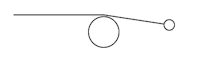
\includegraphics[width = 6 in]{deflection.png}
  \caption{ A diagram showing deflection.
}
\end{figure}

\begin{figure} 
\centering
\label{fig2}
  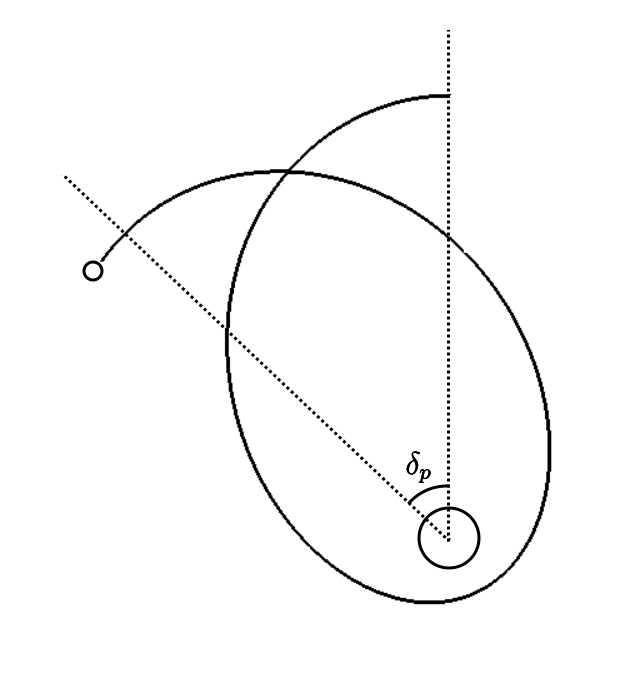
\includegraphics[width = 6 in]{precession.png}
  \caption{ A diagram showing precession, where the orbit does not quite form a closed ellipse.
}
\end{figure}



\begin{figure} 
\centering
\label{fig3}
  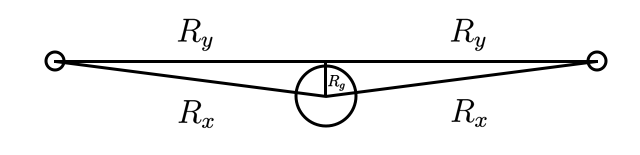
\includegraphics[width = 6 in]{comm.png}
  \caption{ Symmetric communication system, for predicting the Shapiro time delay.
Note that the round-trip time in the absence of the Sun is $\zeta = 4 R_y / c$, and that the time in the presence of the Sun is $\zeta + \delta_{s}$, which is just a little bit longer.
}
\end{figure}


\begin{figure} 
\centering
\label{fig4}
  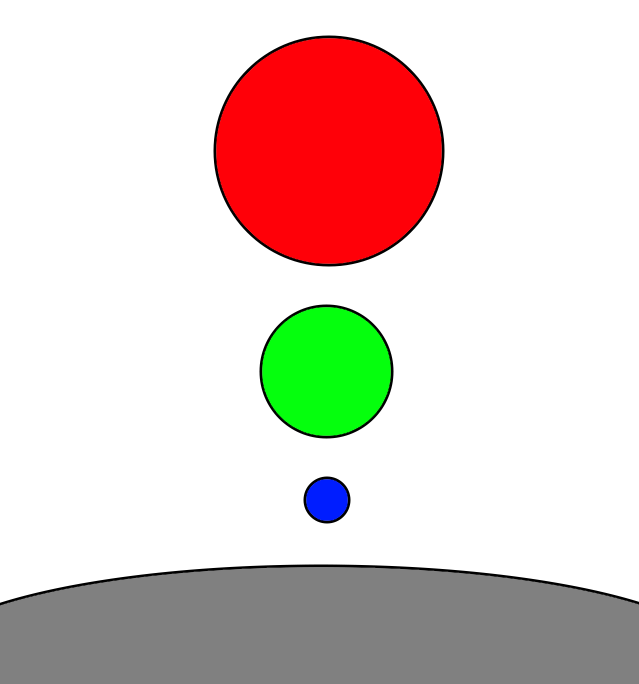
\includegraphics[width = 6 in]{redshift.png}
  \caption{
A diagram showing gravitational redshift.
A blue photon is emitted normal to the surface of a body.
The photon's wavelength increases as it escapes the gravitational field, causing it to redden.
}
\end{figure}




\end{document}









